\chapter{Stationary properties} 


\section{Boundary condition}

To obtain the spectrum of the system it's necessary to find the boundary conditions. As the barrier chemical potential  is the biggest energy parameter of the problem, the wave-functions there are defined by the Hamiltonian:
\begin{gather}
\label{barrier_Hamiltonian}
	H(y)
	=
	\br{
		\frac{p^2}{2m}
		+\mu_b
	}\tau_z,  ~~~~~~~~~-\frac{L}{2}<y<\frac{L}{2}
\end{gather} 

as the low energies are the under consideration, in Sroedinger equation the energy term can be omitted, so $ p_b\approx\pm i \sqrt{2m\mu_b} $. One can solve the problem given by (\ref{barrier_Hamiltonian}) and match the values of the wavefunction and it's derivatives on the left and on the right of the barrier to obtain:
\begin{gather}
	\begin{cases}
	\psi_L + b\partial_y\psi_L=t(\psi_R + b\partial_y\psi_R) \\
	\psi_R - b\partial_y\psi_R=t(\psi_L - b\partial_y\psi_L)
	\end{cases}
\end{gather}

here $ \psi_{L,R}=\psi\br{\mp\frac{L}{2}} $, $ b=\br{{2m\mu_b}}^{-\frac{1}{2}} $ --- the penetration depth for the particle inside th barrier and $ t = e^{-\frac{L}{b} }$ --- the tunneling constant assumed to be small: $ t\ll 1 $. This condition reads, that the size of the barrier $ L $ should be  much bigger that the penetration depth $ b $.

This condition is invariant under the combined action $ L\leftrightarrow R $, $ y\to-y $. To simplify the further analysis one can reverce th direction in the left wire and put both ands of the wires from $ y= \frac{L}{2} $ to $ y=0 $. The boundary condition than becomes:
\begin{gather}
\label{bc_transformed}
\begin{cases}
\psi_L - b\partial_y\psi_L=t(\psi_R + b\partial_y\psi_R) \\
\psi_R - b\partial_y\psi_R=t(\psi_L + b\partial_y\psi_L)
\end{cases}
\end{gather}
This transformation is illustrated on the fig \ref{fig:bctransform}.

The boundary condition (\ref{bc_transformed}) can be rewritten with introducing the spinor $ \Psi=\br{\psi_L, \psi_R}^T $ and Pauli matrices $ \hat{s}_i $ in LR space:
\begin{gather}
	\br{1-t\hat{s}_x}\Psi-\br{1+t s_x}b\pdy\Psi=0
\end{gather}
since for all $ t\ne 1 $ (recall, that $ t\ll1 $) the matrix is $ 1\pm t\hat{s}_x $ in reversible. Multupliing the last equation by $ \br{1-t\hat{s}_x}/\br{1+t^2} $ one obtain:
\begin{gather}
\label{bc_LR_space}
	\br{1-2\tilde{t}\hat{s}_z-\tilde{b}\pdy}\psi=0
\end{gather}
where $ \tilde{t}=\frac{t}{1+t^2} $, $ \tilde{b} = \frac{1-t^2}{1+t^2}b $. In the leading order on $ t $, which corresponds to the tunneling limit, $ \tilde{t}=t $, $ \tilde{b} = b $.
\begin{figure}[H]
	\centering
	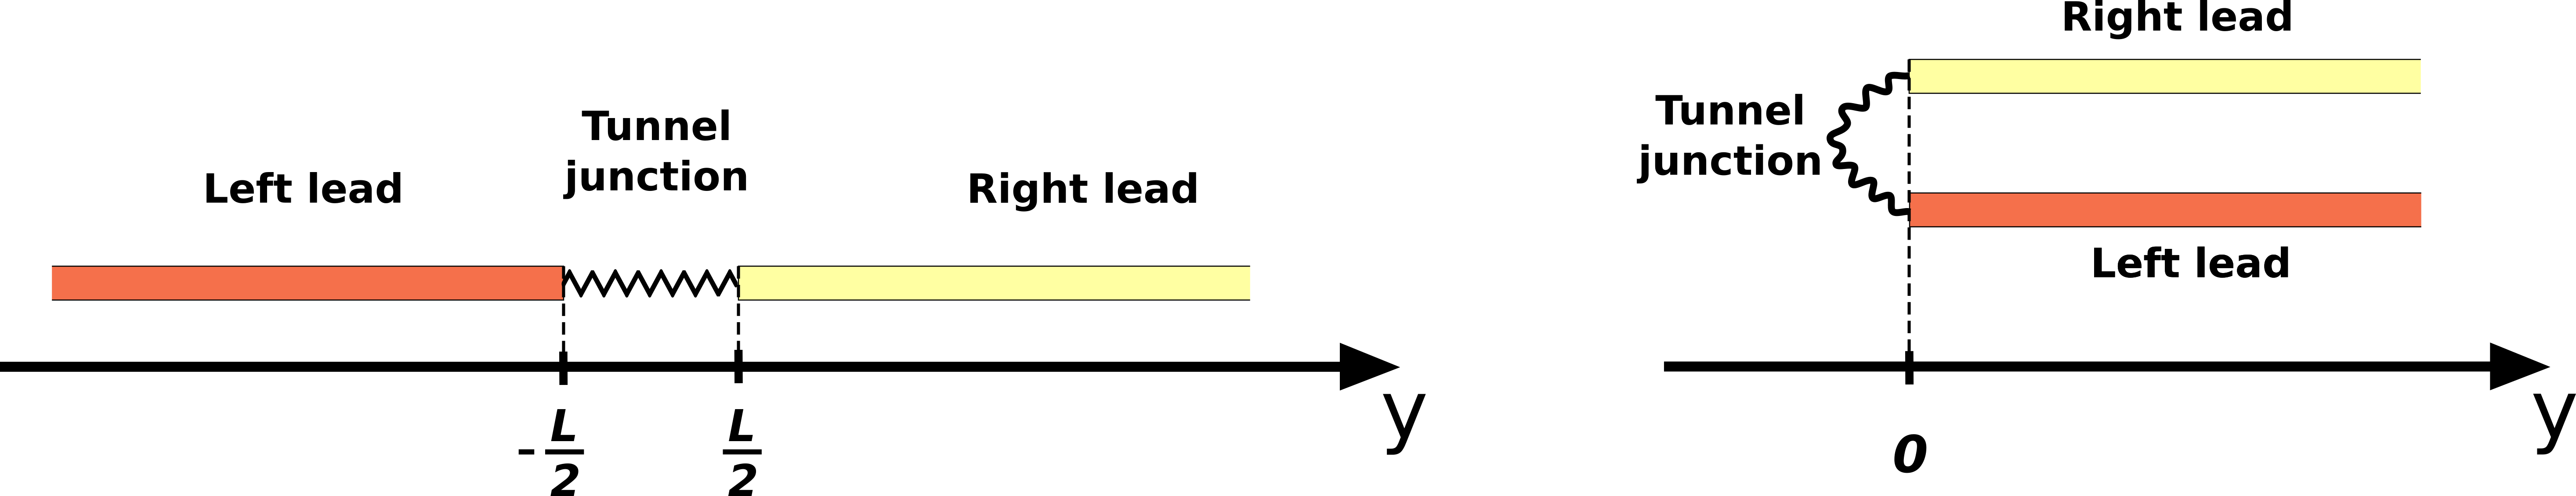
\includegraphics[width=0.9\linewidth]{images/bc_transform}
	\caption{Illustration of switching the direction of left wire}
	\label{fig:bctransform}
\end{figure}

One can argue, that in tunneling limit the second and the third term in (\ref{bc_LR_space}) are much smaller than the first one and should not be taken when the leading order is considered. However, if the second terms is omitted, the leads become efficiently disconnected, and no tunnel effects can be found. The same is true for the third term --- if it's not present, the boundary condition immediately implies $ \Psi\br{0} = 0 $, so the wires become disconnected again.

\section{High momentum modes}  

As was pointed in section \ref{sec:high_and_low_modes}, there are two  shortwave and longwave wavefunctions inside the wire, and the first ones can be described with the Hamiltonian (\ref{short-long_hamiltonian}). However, if one is looking for the localized states, even the longwave modes should be taken decaying. To obtain this, one needs to add a restore superconducting term in (\ref{short-long_hamiltonian}), so the spectrum become gapped and the momenta can get an imaginary part. So, for shortwave modes one should consider a Hamiltonian:
\begin{gather}
\label{high_mods_hamiltonian}
	H=\br{\frac{p^2}{2m}-up\hat{s}_z\sigma_z}\tau_z+\Delta\tau_\phi
\end{gather}
here the multiplier $ \hat{s}_z $ is added in the spin-orbit coupling term, as the direction of the left wire is inverted, so to write a correct Hamiltonian for LR space, one needs to change $ p $ to $ -p $ for the left wire --- which is exactly adding $ -s_z $ multiplier to each momentum.

Denoting $ \eta = \frac{p^2}{2m}-up\hat{s}_z\sigma_z $, one can rewrite (\ref{high_mods_hamiltonian}) as $ H=\eta\tau_z+\Delta\tau_\phi $. As $ \hat{s}_z\sigma_z $ commutes with $ H $ one can treat it as a number, so the dispersion is $ E^2 =\eta^2+\Delta^2 $ (the number corresponding to eigenstate of $ \hat{s}_z $ will be denoted as $ s_z $ while the number, corresponding to the eigenstate of $ \sigma_z $ will be denoted as $ \varsigma_z $). Thus $ \eta=\pm i\sqrt{\Delta^2-E^2} $, as the case $ \abs{E}<\Delta $ is assumed. For momenta\textbf{} one can write the equation:
\begin{gather}
	p^2-2mu s_z \varsigma_z p - 2m \eta =0
\end{gather}
which for shortwave momenta gives $ p_{short}\approx2 mu s_z \varsigma_z + \frac{\eta}{u}s_z\varsigma_z$. Choosing the sign of $ \eta $ in a way, that the wavefunction decays at $ x\to \infty $, one can obtain:
\begin{gather}
\label{short_momentum_decaying}
	p_{short}\approx
	2 mu s_z \varsigma_z 
	+
	i\frac{\sqrt{\Delta^2-E^2}}{u}
\end{gather}


Now the wavefunction can be constructed by putting (\ref{short_momentum_decaying}) into the Schroedinger equation $ \br{\eta\tau_z +\Delta\tau_\phi}\Psi=E\Psi $. The solutions are:
\begin{gather}
	\Psi_{s_z,\varsigma_z}\br{x}
	=
	\begin{pmatrix}
	1
	\\
	e^{i\br{s_z\varsigma_z\gamma+\phi_{s_z}}}
	\end{pmatrix}_{eh}
	e^{2imus_z\varsigma_zx -\frac{\sqrt{\Delta^2-E^2}}{u}x}
	\ket{s_z, \varsigma_z}
\end{gather}
where  $ \ket{s_z, \sigma_z} $ are eigenvectors of matrix $ \hat{s}_z \sigma_z $,  $ \gamma = -\frac{\pi}{2}+\arcsin\frac{E}{\Delta} $ and $ \phi_{1}=\phi_L$, $ \phi_{-1}=-\phi_R $
Thus the longwave part of eqigenstate can be written as:
\begin{gather}
\label{fast_mode_expansion}
	\Psi_{long}
	=
	\sum_{s_z=\pm 1}
	\sum_{\varsigma_z=\pm 1}
	C_{s_z,\varsigma_z}
	\Psi_{s_z,\varsigma_z}\br{x}
\end{gather}
 
  \if 0
\begin{gather}
\begin{pmatrix}
i \hat_z \sigma_z\sqrt{\Delta^2-E^2}-E & \Delta e^{-i\phi_{L,R} s_z} \\
\Delta e^{i\phi_{L,R} s_z} & -i s_z \sigma_z\sqrt{\Delta^2-E^2}-E
\end{pmatrix}
\Psi
=
E\Psi
\end{gather}
\fi


\section{Eliminating longwave modes from boundary condition}
As the Majorana mode acts at low energies, it's expected to be predominantly longwave. This argument is in accord with \cite{Oreg_2010} and \cite{Lutchyn_2010}, where the majorana state was an eigenstate of a linearized Hamiltonian, which is relevant only for longwave physics. So, it's reasonable to eliminate the shortwave modes from the problem, reformulating the boundary condition (\ref{short-long_hamiltonian}).

The wave function can be decomposed in shortwave and  longwave  parts: $ \Psi = \Psi_{short}+\Psi_{long} $. inserting it into the(\ref{short-long_hamiltonian}) and using the fact, that $ p_{long}\ll p_{short} \approx 2mu s_z \sigma_z $, one can obtain at the boundary:
\begin{gather}
	\br{1-2t\hat{s}_x}\Psi_{long}+\br{1-2t\hat{s}_x-2ibum\hat{s}_z \sigma_z}\Psi_{short}=0
\end{gather}
Multipluning by the $ \br{1-2t\hat{s}_x}^{-1} $ and eliminating $ {t^2} $ terms, obtain:
\begin{gather}
	\Psi_{long}
	=
	\br{-1+i\zeta\br{1+2t\hat{s}_x}s_z \sigma_z}\Psi_{short}
\end{gather}
with $ \zeta=2mul $.

Now, using the expansion (\ref{fast_mode_expansion}) and renormalizing the coefficients: $ C_{s_z \varsigma_z}\to-\br{1-i\zeta s_z \varsigma_z}C_{s_z \varsigma_z} $ one can rewrite the boundary condition for $ \varsigma_z $ spin component of the wavefunction as:
\begin{gather}
\Psi_{long,\varsigma_z}
=
\br{1+\frac{2i\zeta t\hat{s}_z\sigma_z}{1+i\zeta \hat{s}_z\sigma_z}}
\sum_{s_z=\pm1}
C_{s_z,\varsigma_z}
		\begin{pmatrix}
	1
	\\
	e^{i\br{s_z\varsigma_z\gamma+\phi_{s_z}}}
	\end{pmatrix}_{eh}
	e^{2imus_z\varsigma_zx -\frac{\sqrt{\Delta^2-E^2}}{u}x}
	\ket{s_z, \varsigma_z}
\end{gather}
This can be  multiplied by $ \br{1+\frac{2i\zeta t\hat{s}_z\sigma_z}{1+i\zeta \hat{s}_z\sigma_z}}^{-1} $, which up to a $ t^2 $ correction yields:

\begin{gather}
\label{bc_projection}
	\br{1-\frac{2i\zeta t\hat{s}_z\sigma_z}{1+i\zeta \hat{s}_z\sigma_z}}
	\Psi_{long,\varsigma_z}
	=
	\sum_{s_z=\pm1}
	C_{s_z,\varsigma_z}
			\begin{pmatrix}
	1
	\\
	e^{i\br{s_z\varsigma_z\gamma+\phi_{s_z}}}
	\end{pmatrix}_{eh}
	e^{2imus_z\varsigma_zx -\frac{\sqrt{\Delta^2-E^2}}{u}x}
	\ket{s_z, \varsigma_z}
\end{gather}

For each $ \varsigma_z $ the above equation can be interpreted as the requirement that the l.h.s. 4-vector (in LR- and eh-spaces) lies in the 2d linear space $ L_{2} $ spanned by the the two vectors in the sum in the r.h.s.. This can be reformulated as the requirement that the l.h.s. be orthogonal to the complementary 2d space $ \overline{L}_{2} $. There are two basic vectors $ \overline{\Psi}_{s_z\varsigma_{z}} $ ($ s_z=\pm1 $) spanning $ \overline{L}_{2} $ for each $ \varsigma_z $:
\begin{gather}
	\overline{\Psi}_{s_z\varsigma_{z}}
	=
	\begin{pmatrix}
	1 \\
	-e^{
		i\br{
			s_z\varsigma_z\gamma
			+
			\phi_{s_z}
			}
		}
	\end{pmatrix}
	\ket{s_z,\varsigma_z}
\end{gather}
Thus one needs to multiply (\ref{bc_projection}) by $ \br{\overline{\Psi}_{+\varsigma_{z}},\overline{\Psi}_{-\varsigma_{z}}} $ from the left and, after all evaluating the matrix produt, find the boundary condition on longwave modes in the form:
\begin{gather}
\label{bc_matrix}
\begin{pmatrix}1 & -e^{-i\left(\sigma_{z}\gamma-\phi_L\right)} & A & -Ae^{-i\left(\sigma_{z}\gamma-\phi_L\right)}\\
A^{*} & -A^{*}e^{i\left(\sigma_{z}\gamma+\phi_R\right)} & 1 & -e^{i\left(\sigma_{z}\gamma+\phi_R\right)}
\end{pmatrix}\Psi_{long, \varsigma_{z}}=0
\end{gather}
here $ A=-\frac{2i\zeta t\sigma_z}{1+i\zeta\sigma_z} $ and the elements are ordered as $ \br{Le,Lh,Re,Rh} $.

When studying wavefunctions in superconductors, it is more convenient to work with zero phase $ \phi $. This can be achieved by gauging the phase difference into the boundary condition. Indeed, suppose $ H_{\phi} $ describes a wire with phase $ \phi $. Then, $ H_{\phi}=U_{\phi}^{\dagger}H_{0}U_{\phi} $ with $ U_{\phi}=\mathrm{diag(1,e^{i\phi})_{eh}} $ and the wave functions are also related via unitary rotation $ \psi_{\phi}=U_{\phi}^{\dagger}\tilde{\psi} $. So the transform $ U^{\dagger}=\mathrm{diag}\br{1,e^{-i\phi_L},e^{-i\phi_L},1,e^{-i\phi_R }}_{Le,Lh,Re,Rh}$  will eliminate all the phases from the rires and put them into boundary condition. Substituting $ \Psi_{long,\varsigma_{z}}=U^{\dagger}\tilde{\Psi} $ into the (\ref{bc_matrix}) one arrives at an even simpler boundary condition on the zero-phase function $ \tilde{\Psi} $:
\begin{gather}
\label{bc_matrix_phases}
\begin{pmatrix}1 & -e^{-i\sigma_{z}\gamma} & A & -Ae^{-i\left(\sigma_{z}\gamma+\varphi\right)}\\
A^{*} & -A^{*}e^{i\left(\sigma_{z}\gamma+\varphi\right)} & 1 & -e^{i\sigma_{z}\gamma}
\end{pmatrix}
\tilde{\Psi}_{long, \varsigma_{z}}=0
\end{gather}
where $ \phi=\phi_R-\phi_L $. Note, that from here it's obvious, that in any physical quantity, calculated with this model, can depend only on phase difference $ \varphi $,  but not on the $ \phi_L $ or $ \phi_R $ separately.

\section{Low momenta and linearized Hamiltonian}

To utilize boundary condition (\ref{bc_matrix}) or (\ref{bc_matrix_phases}), it's necessary to find low momenta wavefunctions in homogenious wire. For this purpose one can use s linearized version of the Hamiltonian (\ref{bulk_Hamiltonian}), like in \cite{Oreg_2010} and \cite{Lutchyn_2010}:
\begin{gather}
\label{linearized_hamiltonian}
		H
	=
	-\mu \tau_z
	+
	u p \sigma_z \tau_z
	+
	B\sigma_x	
	+
	\Delta\tau_x
\end{gather}
here the zero phase $ \phi $ is assumed and $ \mu $ can be equal $ \mu_L $ or $ \mu_R $ depending on the wire considered. As was mentioned before, the nonzero phase can be restored by using $ U_\phi $ matrix. This hamiltonian is valid only for the right wire. To obtain the solution in the left wire one needs to reverse the sign of $ p $ in (\ref{bulk_Hamiltonian}). Instead of doing so, the unitary transform $ \psi_L=\sigma_x\psi_R $ can be utilized, as for (\ref{bulk_Hamiltonian}) $ H\br{-p}=\sigma_x H\br{p}\sigma_x $.

Remembering, that $ \beta=B-\Delta\ll B, \Delta $, one can	treat this Hamiltonian penetratively, decomposing it as $ H=H_0+V_0$:
\begin{gather}
	H_0=
	u p \sigma_z \tau_z
	+
	\Delta
	\br{\sigma_x	
	+
	\tau_x}
\\
V=-\mu \tau_z+\beta\sigma_x
\end{gather}

As $ H_0 $ commutes with $ \sigma_x\tau_x $, it's convenient to rewrite it in the basis of common eigenstates of $ \sigma_x $ and $ \tau_x $. Denoting them as $ \ket{\sigma_x, \tau_x }$ and arranging the order as $  \br{\ket{+, + },\ket{-, - },\ket{+, - },\ket{-, + }} $ one can rewrite $ H_0+V $ as:
\begin{gather}
	H_0
	=
	\begin{pmatrix}
	2\Delta & up & 0 & 0 \\
	up & -2\Delta & 0 & 0\\
	0 & 0 & 0 & up \\
	0 & 0 & up & 0 
	\end{pmatrix}
	~~~~~~~~
	V
	=
		\begin{pmatrix}
	\beta & up & -\mu & 0 \\
	up & -\beta & 0 & v-\mu\\
	-\mu & 0 & \beta & up \\
	0 & -\mu & up & -\beta 
	\end{pmatrix}
\end{gather}
It's easy to see, subspace $ \mathrm{Span}\br{\ket{+, + },\ket{-, - }} $ require no perturbation to obtain the eigenstates in the leading order. Indeed, diagonalizing the upper subblock of $ H_0 $, one finds, that $ E=\sqrt{\br{2\Delta}^2+\br{up}^2} $. When the low energy states are the objects of interest ($ E\sim g_{L,R} $), one finds, that $ p =\pm\frac{i\Delta}{2u} $ in the leading order, and the corresponding eigenstates are $\ket{+, + }\pm i\ket{-, - } $. If

The another two eigenstates are a little bit more complicated. Diaginalizing  the lower subblock of $ H_0 $, one immediately finds, that $ E=\pm up $. This corrseponds to the fact, that $ H_0 $ is the version of $ H $ with a closed gap $ g $  on lower branch (see fig. \ref{fig:spectrum},(e)), so in the zero order this states cannot form anything localized at all. To find them correctly, one needs to take into account the perturbation $ V $ and solve the secular equation using the following ansatz:
\begin{gather}
	\psi = r_1\ket{+, + }+r_2\ket{-, - }+q_{1}\ket{+, - }+q_{2}\ket{-, + }
\end{gather}
with $ r_i\ll q_j $ for all  pairs $ \br{i,j} $. In the leading order (remeber, that both $ E  $ and $ up $ are of the oreder of $ g_{L,R} $ now) this results to a couple of equations:
\begin{gather}
\begin{cases}
	\br{-E+B-\Delta-\frac{\mu^2}{2\Delta}}q_1+up q_2=0
	\\
	u p q_1 + \br{-E-B+\Delta+\frac{\mu^2}{2\Delta}}q_2 =0
\end{cases}
\end{gather}
recall, that at this precision $ g=B-\Delta-\frac{\mu^2}{2\Delta} $ and find $ E^2=g^2+u^2p^2 $.

For this states the momenta are of the order of $ g/u $, so it's reasonably to name them longwave states. Than the states with momenta $ \pm\frac{i\Delta}{2u} $ will be called mediumwave states.
Now it's time to present this wavefunctions in original BdG basis. The expressions here are relevant only for the right lead and for $ E>0 $. To find the wavefunctions in the left lead, the transform $ \psi_L=\sigma_x\psi_R $ can be used, while for finding the negative enrefu states one can utilize electron-hole transform: $ \psi_{E<0}= \tau_y\sigma_yK\psi_{E>0}$ with $ K $ being a complex conjugation operator.

Medium wave states are (propagating version for $ E>2\Delta $ and decaying version for $ E<2\Delta $):
\begin{gather}
	\psi_{medium}=
	\begin{pmatrix}
	1
	\\
	\frac{E\mp\sqrt{E^2-4\Delta^2}}{2\Delta}
	\\
	\frac{E\mp\sqrt{E^2-4\Delta^2}}{2\Delta}
	\\
	1
	\end{pmatrix}
	e^\frac{\pm i x\sqrt{E^2-4\Delta^2}}{u}
	~~~~~
	\psi_{medium}=
	\begin{pmatrix}
	1
	\\
	\frac{E\pm i\sqrt{4\Delta^2-E^2}}{2\Delta}
	\\
	\frac{E\pm, i\sqrt{4\Delta^2-E^2}}{2\Delta}
	\\
	1
	\end{pmatrix}
	e^\frac{\pm  x\sqrt{4\Delta^2-E^2}}{u}
\end{gather}

However in the most part of this work the low energy version $\psi_{medium}=
\br{
1,
\pm i,
\pm i,
1
}^T
e^{\pm\frac{\Delta x}{2u}}  $

will be used.

Longwavestates (for energies $ E\sim g_{L,R} $, for $ E>g $ and $ E<g $ respectfully):
\begin{gather}
		\psi_{long}
=
\begin{pmatrix}
1\\
\frac{E\mp \sqrt{E^2-g^2}}{g}\\
-\frac{E\mp \sqrt{E^2-g^2}}{g}\\
-1
\end{pmatrix}
e^{\pm\frac{ix\sqrt{E^2-g^2}}{u}}
~~~~~~
	\psi_{long}
	=
	\begin{pmatrix}
	1\\
	\frac{E\pm i\sqrt{g^2-E^2}}{g}\\
	-\frac{E\pm i\sqrt{g^2-E^2}}{g}\\
	-1
	\end{pmatrix}
	e^{\pm\frac{x\sqrt{g^2-E^2}}{u}}
\end{gather}